\section{Komponentenschnittstellen}

%3.1 Datentypen
\subsection{\textit{Datentypen}}
Die in Abbildung \ref{KomponentenschnittstellenDiagramm} dargestellten Datentypen werden von den Schnittstellen der eingeführten Komponenten verwendet. 

Die Aufgabe des Datentyps \emph{SensorData} ist primär, die Koordination mit dem Server zu unterstützen, um festzustellen, inwieweit eine Zielposition gut erreicht werden kann. Dazu besitzt er als Attribute die Orientierungsrichtung im Koordinatensystem, den Batteriestatus und zuletzt Attribute der Datentypen \emph{Position} und \emph{Destination}. \emph{Position} besitzt wiederum die Koordinaten x und y, die einen beliebigen Punkt im Bereich des Einsatzgebietes des Roboters darstellen. Um Redundanz zu vermeiden sind \emph{Destination} und \emph{Position} über keine zusätzliche Klassendiagrammbeziehung verknüpft. Zielpunkte erben von \emph{Position} und existieren zur Spezifikation, um welche Art Zielpunkt es sich handelt: Also zum Beispiel eine allgemeine \emph{Destination} oder den \emph{Charger}.
	
	\begin{figure}[H]
		\centering
		\includegraphics[width=0.75\textwidth]{img/3-Zusatzklassen}
		\caption{Datentypen, die in Komponentenschnittstellen verwendet werden}
		\label{KomponentenschnittstellenDiagramm}
	\end{figure}
	\pagebreak

%3.2 Interfaces
\subsection{\textit{Interfaces}}
	%3.2.1 ISensorData
	\subsubsection{\textit{ISensorData}}
	Dieses \textit{Interface} wird vom \textit{Robot} angeboten, um dem Server alle Sensordaten zu senden. Der Server kann anhand diesen jederzeit feststellen, in welchem Zustand sich der \textit{Robot} befindet um diesem dann eine \textit{Task} zuzuweisen.
	\begin{figure}[H]
	\centering
	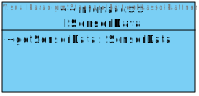
\includegraphics[width=0.75\textwidth]{img/1-Entwurf-3-1_ISensorData}
	\caption{\textit{Interface} ISensorData}
	\label{ISensorData}
	\end{figure}
	
	%3.2.2 ITask
	\subsubsection{\textit{ITask}}
	Dieses \textit{Interface} wird vom \textit{Robot} angeboten, um Tasks zu erhalten. Der Server kann somit ohne Probleme \textit{Tasks} dem \textit{Robot} zuweisen. Hierbei findet eine Unidirektionale Kommunikation zwischen Server und Robot statt.
	\begin{figure}[H]
	\centering
	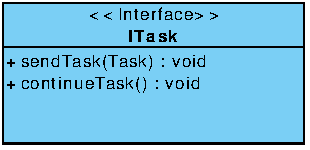
\includegraphics[width=0.75\textwidth]{img/1-Entwurf-3-1_ITask}
	\caption{\textit{Interface} ITask}
	\label{ITask}
	\end{figure}
